\documentclass{article}
\usepackage[utf8]{inputenc}
\usepackage{graphicx}
\usepackage{float}
\usepackage{amsmath}
\usepackage{amssymb}
\usepackage{listings}
\usepackage{color}
\usepackage{siunitx}
\usepackage{comment}
\usepackage{hyperref}
\usepackage{enumitem}
\usepackage{cite}
\usepackage{environ}
\usepackage{caption}
\usepackage{subcaption}
\newcommand\tab[1][1cm]{\hspace*{#1}}

\makeatletter
\NewEnviron{widerequation}{%
  \begin{equation*}
  \sbox\z@{\let\label\@gobble$\displaystyle\BODY$}
  \makebox[\textwidth]{%
    \begin{minipage}{\dimexpr\wd\z@+3em}
    \vspace{-\baselineskip}
    \begin{equation*}
    \BODY
    \end{equation*}
    \end{minipage}%
  }
  \end{equation*}
}
\makeatother

\definecolor{codegreen}{rgb}{0,0.6,0}
\definecolor{codegray}{rgb}{0.5,0.5,0.5}
\definecolor{codepurple}{rgb}{0.58,0,0.82}
\definecolor{backcolour}{rgb}{0.95,0.95,0.92}
 
\lstdefinestyle{mystyle}{
    backgroundcolor=\color{backcolour},   
    commentstyle=\color{codegreen},
    keywordstyle=\color{magenta},
    numberstyle=\tiny\color{codegray},
    stringstyle=\color{codepurple},
    basicstyle=\footnotesize,
    breakatwhitespace=false,         
    breaklines=true,                 
    captionpos=b,                    
    keepspaces=true,                 
    numbers=left,                    
    numbersep=5pt,                  
    showspaces=false,                
    showstringspaces=false,
    showtabs=false,                  
    tabsize=2
}

\lstset{style=mystyle}

\title{TTK22 Software Toolchain for Networked Vehicle Systems Project}
\author{Henning Ødeby Karlsen}
\date{November 2020}

\begin{document}

\maketitle

%
% GRAPHICS
%

% \begin{figure}[H]
%     \centering
%     \includegraphics[width=8cm]{MATLAB/bike.png}
%     \caption{The bike model, from the assignment paper}
%     \label{fig:pendulum_on_cart}
% \end{figure}

%
% MATRIX ADDITION ETC
%
% $$ M
% \begin{bmatrix}
%     \ddot\phi\\
%     \ddot\delta
% \end{bmatrix}
% +Cv_0
% \begin{bmatrix}
%     \dot\phi\\
%     \dot\delta
% \end{bmatrix}
% +(K_0+K_2v^2_0)
% \begin{bmatrix}
%     \phi\\
%     \delta
% \end{bmatrix}
% =
% \begin{bmatrix}
%     0\\
%     T
% \end{bmatrix}
% $$

%
% EQUATIONS
%

% $$ \ddot\phi = -\frac{\dot\phi Cv_0 }{M} - \frac{(K_0+K_2v^2_0)\phi}{M}$$
% $$ \ddot\delta = \frac{T}{M} -\frac{\dot\delta Cv_0 }{M} - \frac{(K_0+K_2v^2_0)\delta}{M}$$

%$$ 
% A =
% \begin{bmatrix}
%     0 && 0 && 1 && 0\\
%     0 && 0 && 0 && 1\\
%     - \frac{(K_0+K_2v^2_0)}{M} && 0 && -\frac{Cv_0 }{M} && 0\\
%     0 && - \frac{(K_0+K_2v^2_0)}{M} && 0 && -\frac{Cv_0 }{M} 
% \end{bmatrix}
% $$
%$$ 
% A =
% \begin{bmatrix}
%     0 && 0 && 1 && 0\\
%     0 && 0 && 0 && 1\\
%     - \frac{(K_0+K_2v^2_0)}{M} && 0 && -\frac{Cv_0 }{M} && 0\\
%     0 && - \frac{(K_0+K_2v^2_0)}{M} && 0 && -\frac{Cv_0 }{M} 
% \end{bmatrix}
% $$

%
% 3x3 MATRIX
%

% $$ 
% A =
% \begin{bmatrix}
%     0 && 0 && 1 && 0\\
%     0 && 0 && 0 && 1\\
%     - \frac{(K_0+K_2v^2_0)}{M} && 0 && -\frac{Cv_0 }{M} && 0\\
%     0 && - \frac{(K_0+K_2v^2_0)}{M} && 0 && -\frac{Cv_0 }{M} 
% \end{bmatrix}
% $$

%
% CODE 
%

% \lstinputlisting[language=matlab]{MATLAB/output.m}
% \lstinputlisting[language=matlab, firstline=94, lastline=113]{MATLAB/bike.m}

%
% TABLES
%

% https://no.overleaf.com/learn/latex/Tables

% \begin{center}
%     \begin{tabular}{ |c|c|c| } 
%      \hline
%      cell1 & cell2 & cell3 \\ 
%      cell4 & cell5 & cell6 \\ 
%      cell7 & cell8 & cell9 \\ 
%      \hline
%     \end{tabular}
%\end{center}

%
% TEXT FORMATTING
%

% https://www.overleaf.com/learn/latex/bold,_italics_and_underlining

%
% LISTS WITH a,b,c etc.
%

% \begin{enumerate}[label=(\alph*)]
%     \item What is the size of the training set used?\\
%     \textit{\textbf{Answer:} 300}
%     \item Which class had the highest number of errors?\\
%     \textit{\textbf{Answer:} Class 9 out of 10 classes, with 10 errors, assuming an error is anything that lies outside of the diagonal, where correct class = predicted class}
%     \item What was the overall percentage correct?\\
%     \textit{\textbf{Answer:} Overall correct percentage was 86.667\% }    
% \end{enumerate}

%
% CASES (Squig over flere linjer)
%

% \begin{cases}
%     \pi^{d/2}/(d/2)!, &  d \text{ even}\\
%     2^d\pi^{(d-1)/2}\frac{d-1}{2}!/d!, &  d \text{ odd}\\
% \end{cases} 

%
% Footnote
%

% \footnote{Denne teksten blir stående nede, også kommer det et tall der dette står.}
% Har litt andre funksjoner også https://www.overleaf.com/learn/latex/footnotes

%
% Hyperlenker https://www.overleaf.com/learn/latex/hyperlinks
%

% \href{URL}{tekst}



\newpage
\section{Approach}
For this project, I wanted to see what would be required for SINTEF's JavaScript Graphical User Interface, Aqueous, to communicate with DUNE, instead of the FhSim it is set up to communicate.
I also wanted to leave DUNE as it is, such that any changes needed should be done on Aqueous.
\subsection{Aqueous}
Aqueous is used as the interface between the operator and the control system (FhSim) of one of SINTEF's ROVs.
It was originally developed by students in the course TDTin the JavaScript framework React, and 
The GUI has two components. The first is a Video HUD for displaying the video feed from the ROV as well as visualize the location of the ROV. 
The second is a control view for visualizing the current control situation, as well as issuing some controls. 
In the control view, the user can switch between three different modes: NF (NetFollowing), DP (DynamicPositioning) and Manual.
The manual control and changing of biases in the other modes are done either by a gamepad or the keyboard. 

\begin{figure}[H]
    \centering
    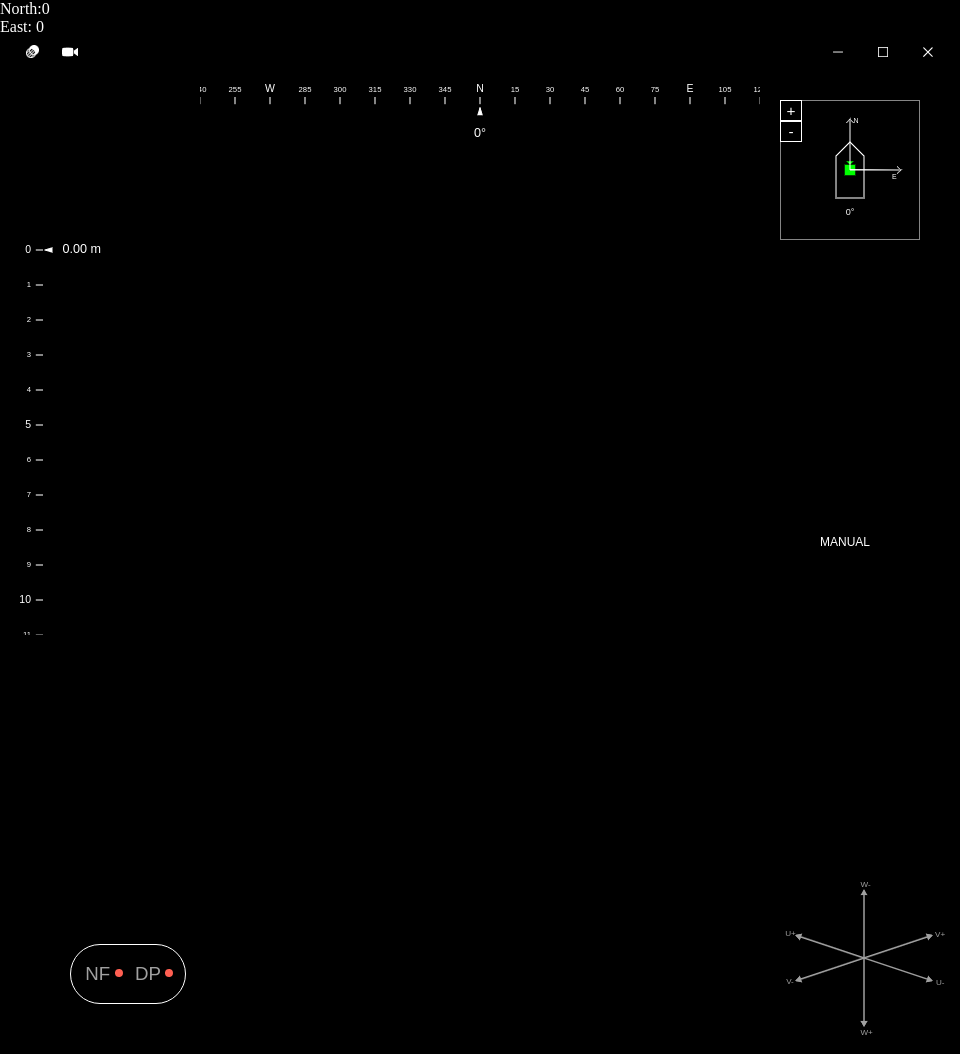
\includegraphics[width=0.75\textwidth]{AqHUD.png}
    \caption{The video HUD. When no ROV/video is connected, the screen is black}
    \label{fig:HUD}
\end{figure}

\begin{figure}[H]
    \centering
    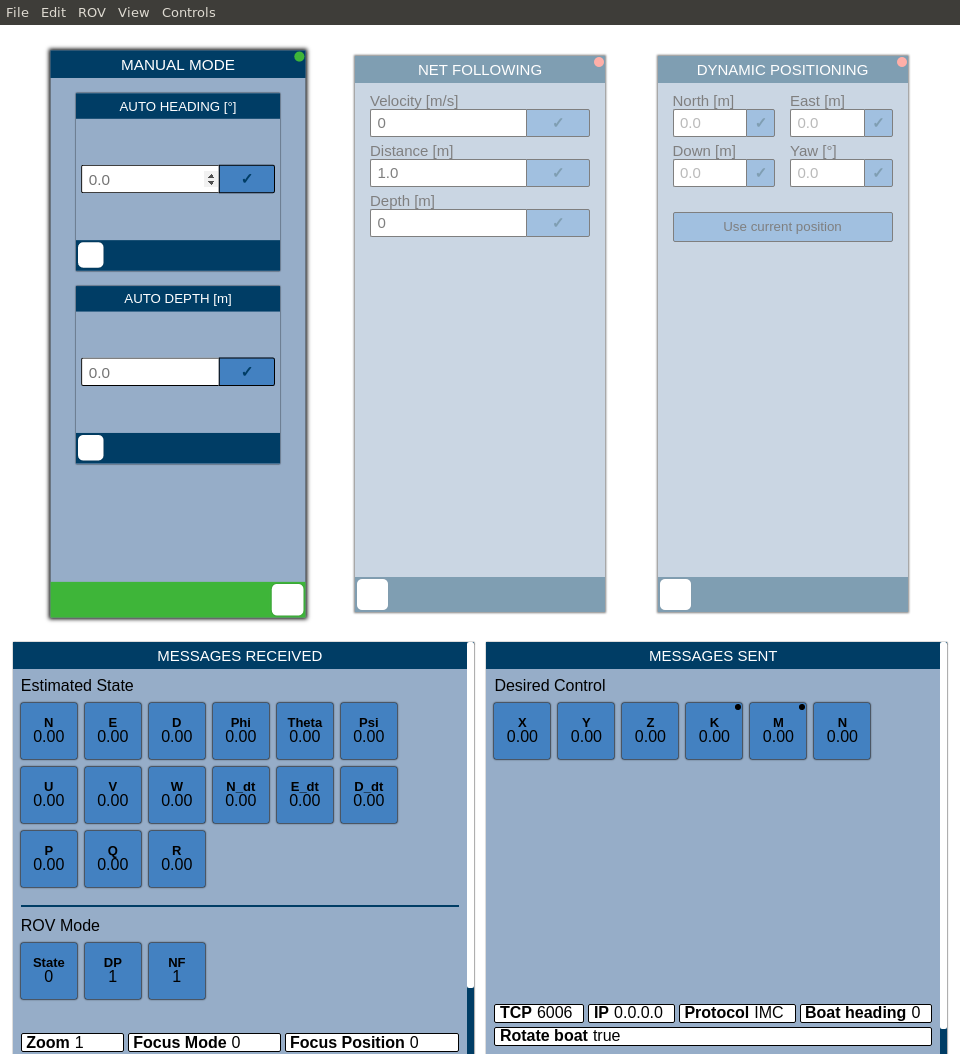
\includegraphics[width=\textwidth]{AqControl.png}
    \caption{The control view when no ROV is connected.}
    \label{fig:control}
\end{figure}
\noindent
The relevant parts of Aqueous for this project is the communication with FhSim, which I will look into changing in this project, such that it can be used to communicate with DUNE.
\subsection{Existing Communcations}
Aqueous is already set up to use IMC for communication with FhSim, but it uses a few custom messages, and does not follow the same set of communication rules as DUNE.
I was told by people at SINTEF that Aqueous would not work "out of the box" with DUNE. 
So I started with trying to get them connected through TCP. 
After finding the right addresses I was able to get a connection between them, but Aqueous instantly crashed as it was not prepared to receive unknown messages.
\subsection{Receiving Messages from DUNE}
I started by looking into the way Aqueous receives these messages, such that I could add support for the different messages that DUNE sends, and discard the unwanted messages.
After some debugging and tinkering, I was able to see what message IDs the LAUV Xplore 2 control system sent. 
And after looking up the most common ones I decided to attempt to decode the estimated state message. How this was done can be found in \autoref{org} and the results in \autoref{res}
\subsection{Sending Messages to DUNE}
Receiving, decoding, and using a message is not enough for Aqueous to use DUNE as its control system. 
I also needed to send messages that DUNE can interpret and use for control of an ROV or some other autonomous vehicle.
Initially, I had to see if DUNE received the messages I sent and if it handled them in any way.
This turned out to be challenging as DUNE is a large and interconnected software system. 
It took me some time and help to find the right location where the messages were received and decoded or discarded.
Without changing anything in Aqueous, all the messages sent were just discarded.
I first started trying to send the desired control message, as it was already implemented in Aqueous and FhSim.
However, it turned out that DUNE expected a structure of messages. For example, DUNE requires control loops to be enabled before it will handle any desired control messages.

\section{Organization}\label{org}
\subsection{Decoding and Handling Estimated State}
Aqueous already has an estimated state message, but it is customized such that it is relative to the mother ship.
Aqueous also does not use the entire estimated state message, but only the positions and rotations.
When Aqueous receives a message it first decodes the heading and finds the message ID from IMC. 
It then maps the rest of the message to a predefined data structure.
I made a copy of the data structure for the custom estimated state and altered it such that it is identical to the estimated state that DUNE sends.
The data structure can be seen in the appendix, \autoref{EstStateDS}.
This data is then saved in a global variable which, among other things, is used for displaying the position of the ROV.
This can be seen in \autoref{SaveESD}

\subsection{Sending Desired Control and Debugging from DUNE}
As the desired control message was already ready to use in Aqueous, I tried sending it to DUNE.
At first, it seemed like nothing happened, and that the message was simply discarded.
But after some digging in DUNE, I was able to see that the message was in fact decoded and handled.
However, it was not used for control of the vehicle. 
I was able to find out that I first needed to send a Control Loop message to enable control loops, 
which then again should activate the Allocate task (which handles desired control) in DUNE.

\subsection{Sending the Control Loop Message}
To encode and send an IMC message in Aqueous I needed to build a data structure and populate it with data.
These can be found in the appendix, respectively \autoref{ControlLoopDS} and \autoref{ControlLoopPop}





\section{Results}\label{res}
\subsection{DUNE to Aqueous}
Receiving and decoding the estimated state message worked, and I was able to use and display this information in Aqueous.
This was only done for the fairly simple estimated state message, but it should not be hard to implement other messages.
One thing that should be noted is the possibility that messages need to be adapted to work as intended in Aqueous.
An example of this is the relativity of the custom estimated state message that Aqueous and FhSim used in the first place.
In Aqueous you expect to see the position relative to the mother ship, 
meaning that some transformation of coordinates would need to be done in order to achieve the same when using DUNE.
Another thing that would need to be completely redone is the video streaming functionality. For simulation purposes, however, this is not relevant.

\begin{figure}[H]
  \centering
  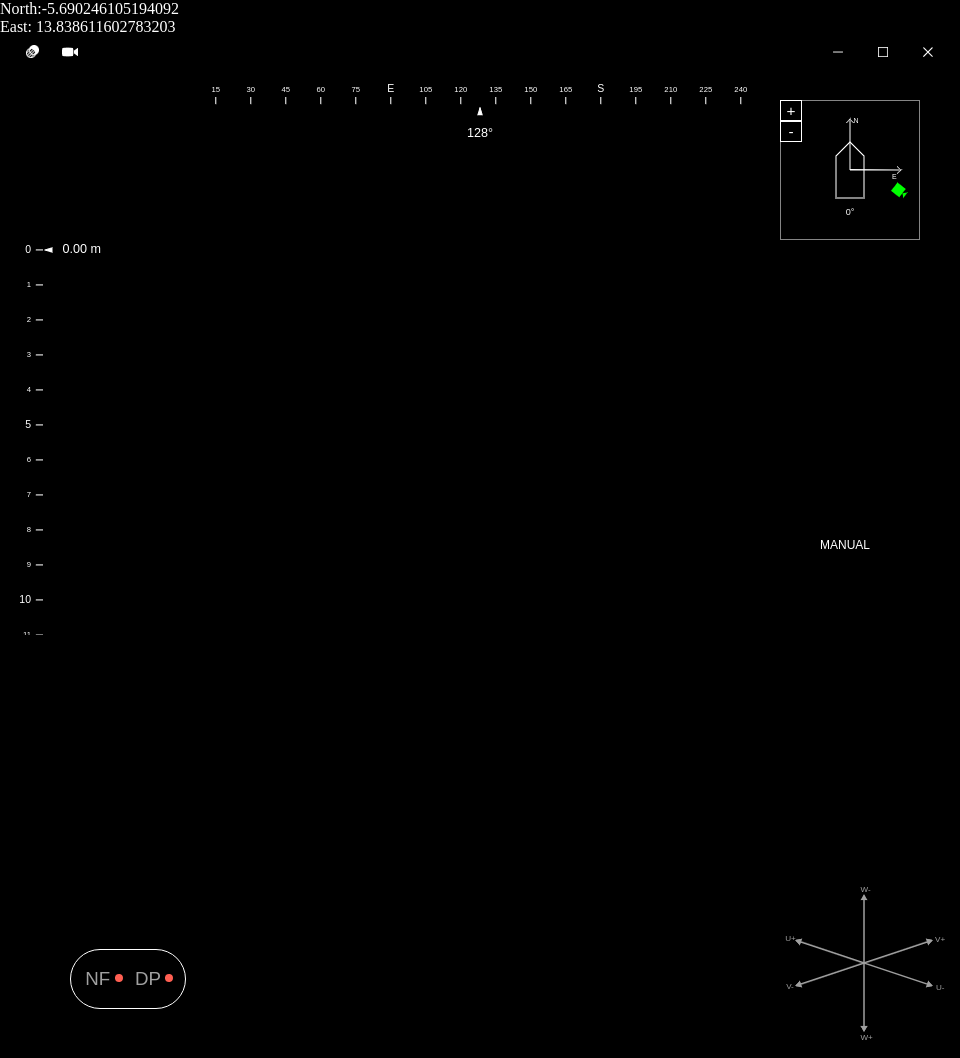
\includegraphics[width=\textwidth]{AqHUDConnected.png}
  \caption{The video HUD when connected to DUNE, and moved from Neptus. Note the little green box indicating the ROV, as well as the position.}
  \label{AqHudDUNE}
\end{figure}
\begin{figure}[H]
  \centering
  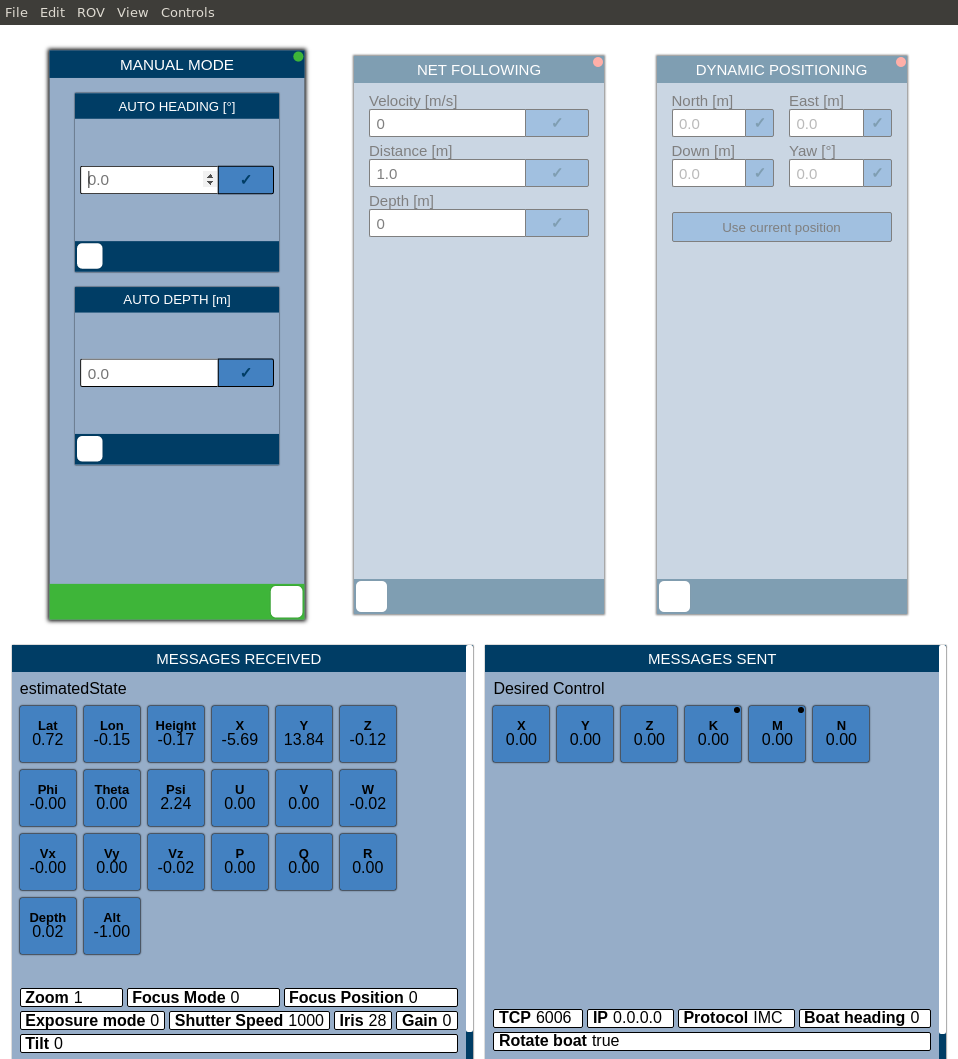
\includegraphics[width=\textwidth]{AqControlConnected.png}
  \caption{The control view when connected to DUNE, and moved from Neptus. Note the positions in the lower left corner.}
  \label{AqControlDUNE}
\end{figure}

\subsection{Aqueous to DUNE}
I was not able to get the desired control message working properly. 
This is probably due to the bitfield flags being implemented in the wrong way, or some error in the destination entity or similar.
With some hours of debugging this problem would probably have been fixable, but I had to limit the amount of time I spent on this project.
I also tried to implement and send the desired path message, but something went wrong with the values in the message.
The control loop message, however, worked as intended, and I was able to activate the Allocator task.
Again, it should be fairly straight forward to implement simple messages.
However, Aqueous and FhSim includes other advanced functions such as net-following.
These would need to either be transformed and translated into standard IMC messages or be implemented as modes in DUNE.
For net-following, this might be challenging as it relies on DVL measurements.

\subsection{General}
For Aqueous to communicate with DUNE, such that DUNE can be used to control an autonomous vessel, there are a few things that must be implemented.
All the messages from DUNE that one wishes to use in Aqueous need to be translated, implemented, and handled. 
These could be messages similar to what FhSim already sends to Aqueous (i.e. customEstimatedState/customGoTo) 
or it could be other messages previously not used in Aqueous (i.e. NavigationUncertainty/VehicleState).
\\~\\
Any functionality in Aqueous must be implemented in such a way that it can be broken down into standard IMC messages and sent to DUNE.
This requires that the functionality is compatible with DUNE, and the vehicle used in DUNE.
\\~\\
One major thing that would greatly reduce the challenges of this communication, would be an implementation of SINTEF's ROV in DUNE.
This would allow for things such as the front-facing DVL to be implemented.
As well as reducing the need for "extra" messages/different structures, such as encountered with the control loops message.
\\~\\
Another thing making this communication challenging, is the different structure of the control system in FhSim and DUNE. 
While DUNE is built to receive and execute different plans or do low-level control of the vessel, 
the current setup in FhSim has a few different modes that are not necessarily configured as plans.
A change in this would make a transition to DUNE easier, but one might not be able to retain the required functionality. 





\section{Appendix}\label{appendix}
\subsection{Estimated State Metadata Data Structure}\label{EstStateDS}
\lstinputlisting[language=java]{estimatedStateMetadata.js}
\newpage
\subsection{Saving Estimated State Data}\label{SaveESD}
\lstinputlisting[language=java]{saveData.js}

\subsection{Control Loop Metadata Data Structure}\label{ControlLoopDS}
\lstinputlisting[language=java]{clMetadata.js}

\subsection{Populating the Control Loop object with data}\label{ControlLoopPop}
\lstinputlisting[language=java]{clPop.js}


% \bibliography{references.bib}{}
% \bibliographystyle{abbrv}
\end{document}